\documentclass{article}
\usepackage[utf8]{inputenc} 
\usepackage[T1]{fontenc}
\usepackage[french]{babel} 
\usepackage{graphicx}
\usepackage[top=2cm, bottom=2cm, left=3cm, right=3cm]{geometry}
\usepackage{amsthm}
\usepackage{amsmath}
\usepackage{amssymb}
\usepackage{mathrsfs}
\usepackage{stmaryrd}
\usepackage{appendix}
\usepackage{dsfont}
\usepackage{hyperref}
\usepackage{caption}
\usepackage{subcaption}
\usepackage{xcolor}
\usepackage{dsfont}
\usepackage{listings}
\usepackage{pgf, tikz}
\usetikzlibrary{arrows}

\definecolor{codeblue}{rgb}{0.2,0.2,0.9}
\definecolor{codegreen}{rgb}{0.,0.5,0.2}
\definecolor{codegray}{rgb}{0.5,0.5,0.5}
\definecolor{codepurple}{rgb}{0.58,0,0.82}
\definecolor{backcolour}{rgb}{0.95,0.95,0.92}

\lstdefinestyle{mystyle}{
    language=Python,
    backgroundcolor=\color{backcolour},   
    commentstyle=\color{codegreen},
    keywordstyle=\color{codeblue},
    numberstyle=\tiny\color{codegray},
    stringstyle=\color{codepurple},
    basicstyle=\ttfamily\footnotesize,
    breakatwhitespace=false,         
    breaklines=true,                 
    captionpos=b,                    
    keepspaces=true,                 
    numbers=left,                    
    numbersep=5pt,                  
    showspaces=false,                
    showstringspaces=false,
    showtabs=false,                  
    tabsize=2
}

\lstset{style=mystyle}

% \allowdisplaybreaks[1]

\newcommand*{\ZnZ}[1]{\mathbb{Z}/#1\mathbb{Z}}
\newcommand*{\iintervalle}[2]{[\![#1,#2]\!]}
\newcommand*{\N}{\mathbb{N}}
\newcommand*{\Z}{\mathbb{Z}}
\newcommand*{\Q}{\mathbb{Q}}
\newcommand*{\R}{\mathbb{R}}
\newcommand*{\C}{\mathbb{C}}
\newcommand*{\K}{\mathbb{K}}
\newcommand*{\Proba}{\mathbb{P}}
\newcommand*{\Mat}{\mathrm{Mat}}
\newcommand*{\Lcal}{\mathcal{L}}
\newcommand*{\Mcal}{\mathcal{M}}
\newcommand*{\Pcal}{\mathcal{P}}
\newcommand*{\perm}[1]{\mathfrak{S}_{#1}}
\newcommand*{\detb}[1]{\mathrm{det}_{\underline{#1}}}
\newcommand*{\scal}[2]{\langle #1, #2 \rangle}
\newcommand*{\norme}[1]{\left \Vert #1 \right \Vert}
\newcommand*{\normet}[1]{\left\vert\kern-0.25ex\left\vert\kern-0.25ex\left\vert #1 
\right\vert\kern-0.25ex\right\vert\kern-0.25ex\right\vert}
\newcommand*{\dd}[1]{\mathrm{d}#1}
\newcommand*{\E}{\mathbb{E}}
\newcommand*{\V}{\mathbb{V}}
\newcommand*{\cov}[2]{\mathrm{cov}(#1, #2)}

\DeclareMathOperator*{\ppcm}{ppcm}
\DeclareMathOperator*{\pgcd}{pgcd}
\DeclareMathOperator*{\rad}{rad}
\DeclareMathOperator*{\ord}{ord}
\DeclareMathOperator*{\id}{id}
\DeclareMathOperator*{\dom}{dom}
\DeclareMathOperator*{\rg}{rg}
\DeclareMathOperator*{\tr}{tr}
\DeclareMathOperator*{\e}{e}
\DeclareMathOperator*{\Vect}{Vect}
\DeclareMathOperator*{\Ker}{Ker}
\DeclareMathOperator*{\im}{Im}
\DeclareMathOperator*{\GL}{GL}

\let \epsilon \varepsilon 
\let \vec \overrightarrow

\theoremstyle{definition}
\newtheorem{definition}{Définition}
\theoremstyle{remark}
\newtheorem{remarque}{Remarque}
\theoremstyle{plain}
\newtheorem{theorem}{Théorème}
\theoremstyle{definition}
\newtheorem*{lemma}{Lemme}
\newtheorem*{example}{Exemple}


\title{TIPE : La reconstruction tomographique}
\author{Damien ROUCHOUSE}
\date{2021-2022}

\begin{document}
\maketitle

\section*{Introduction}
La tomographie est un ensemble de techniques visant à reconstruire l’intérieur d’un objet sans y avoir accès. 
C'est notamment le principe utilisé par les scanners à rayons X. La tomographie discrète étudie le cas très particulier 
où le nombre d’axes de projection est limité et éventuellement où l'objet est une image discrète.

\section{Transformée de Radon : Intérêt pratique}
\subsection{Définition de la transformée de Radon}
\begin{definition}
    Soit $f : \R^2 \longrightarrow \R$ une fonction telle que $v \in \R \mapsto f(u \cos{\theta} - v \sin{\theta}, u \sin{\theta} + v \cos{\theta})$ est intégrable. 
    On définit la transformée de Radon par rapport à la droite de paramètre $(u, \theta)$ par : 
    $$R[f](u,\theta) = \int_{-\infty}^{+\infty} f(u \cos{\theta} - v \sin{\theta}, u \sin{\theta} + v \cos{\theta}) \dd v $$
\end{definition}

\subsection{Intérêt pratique}
\noindent La loi de Beer-Lambert nous assure que : 
$$I(u,\theta) = I_0(u,\theta) \cdot \exp\left(-R[f](u,\theta)\right)$$
ce qui fait le lien entre la transformée de Radon et l'imagerie médicale. 
\noindent On accède ainsi à la transformée de Radon $R[f]$ à partir de la mesure de $I$. Seulement, le but principal est d'accéder à $f$. Il faut alors expliciter une démarche pour 
passer de la transformée de Radon $R[f]$ à $f$ : c'est le problème de la reconstruction tomographie.

\section{Reconstruction tomographique : Transformée de Radon inverse}
\subsection{Utilisation des sinogrammes}
En pratique les machines à rayons X donnent accès aux valeurs de $R[f](u,\theta)$ par une représentation en niveau de gris dans le plan d'axes $\theta$ et $u$.
On appelle cette représentation : sinogramme. Le but est de reconstruire l'objet à partir de son sinogramme. On donne ci-dessous un exemple de sinogramme : 
\begin{figure}[h]
    \centering
    \begin{subfigure}{0.3\textwidth}
        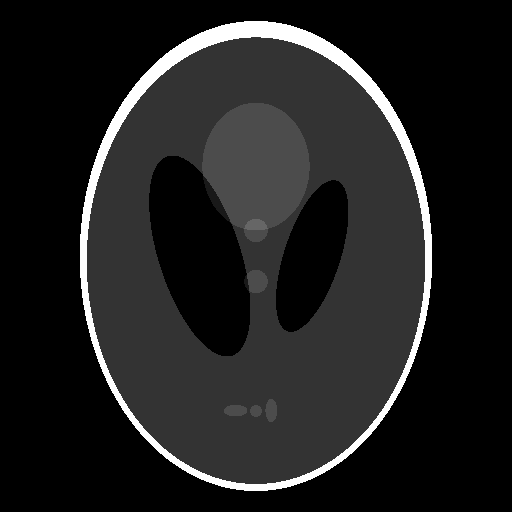
\includegraphics[width=\textwidth]{original.png}
        \caption{Objet à reconstruire}
    \end{subfigure}
    \qquad \qquad 
    \begin{subfigure}{0.17\textwidth}
        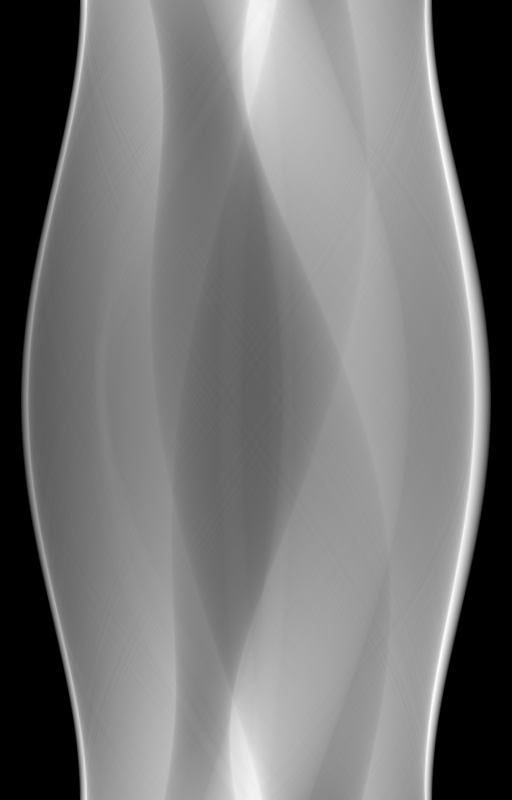
\includegraphics[width=\textwidth]{sinogram.png}
        \caption{Sinogramme de l'objet}
    \end{subfigure}
\end{figure}
\newpage
\subsection{Transformée de Fourier}
\begin{definition}[Transformée de Fourier]
        En dimension 1 : soit $f : \R \longmapsto \R$ une fonction intégrable, on définit la transformée de Fourier par : 
        $$\forall \nu \in \R, \; \widehat{f}(\nu) = \int_{\R} f(t)\mathrm{e}^{-2 i \pi \nu t } \dd t$$  
        En dimension 2 : soit $f : \R^2 \longmapsto \R$ une fonction intégrable, on définit la transformée de Fourier par : 
        $$\forall (u,v) \in \R^2, \; \widehat{f}(u,v) = \int_{\R^2} f(x,y) \mathrm{e}^{-2 i \pi (ux + vy)} \dd x \dd y $$
\end{definition}
\begin{theorem}[Théorème d'inversion de Fourier]
        Sous certaines hypothèses supposées vérifiées dans le cadre de notre étude, on peut accéder à $f$ par inversion de sa transformée de Fourier.  \\
        En dimension 1 : $$\forall t \in \R, f(t) = \int_{\R} \widehat{f}(\nu)\mathrm{e}^{2i\pi \nu t} \dd \nu$$
        En dimension 2 : $$\forall (x,y) \in \R^2, f(x,y) = \int_{\R^2} \widehat{f}(u,v)\mathrm{e}^{2i\pi (ux + vy)} \dd u \dd v$$
\end{theorem}
\begin{proof}
    admis. 
\end{proof}
\begin{remarque}
Il est par exemple suffisant que $f$ soit dans l'espace de Schwartz $\mathcal{S}(\R^d) \; (d \in \{1,2\})$ où : 
$$\mathcal{S}(\R) = \{f \in \mathcal{C}^{\infty} : \forall (n,m) \in \N, x \mapsto x^{n} f^{(m)}(x) \text{ bornée} \}$$
$$\mathcal{S}(\R^2) = \{f \in \mathcal{C}^{\infty} : \forall (p,q,n,m) \in \N^4, (x,y) \mapsto x^{p}y^q \partial_x^n \partial_y^m f(x,y) \text{ bornée}\}$$
\end{remarque}

\subsection{Inversion analytique}
Nous allons voir dans cette section l'inversion théorique de la transformée de Radon pour retrouver l'objet à partir de son sinogramme.
\begin{theorem}[Théorème de la coupe Centrale]\label{coupe}
Soient $\theta \in [0,\pi[$ et $u \in \R$ et $f : \R^2 \longrightarrow \R$ la fonction caractéristique de notre objet. En notant $p_{\theta} : t \in \R \longmapsto R[f](t,\theta)$ on a : 
$$\widehat{p_{\theta}}(u) = \widehat{f}(u \cos \theta , u \sin \theta)$$    
où  $\; \widehat{.}\;$ est l'opérateur de transformée de Fourier. 
\end{theorem}
\begin{proof}
    On admettra le théorème de Fubini et le théorème de changement de variable pour les fonctions de $\R^2$ dans $\R$. 
    \begin{align*}
        \widehat{p_{\theta}}(u) = \int_{\R} p_{\theta}(t)\; \mathrm{e}^{-i u t} \; \dd t &= \int_{\R} \left(\int_{\R} f(t \cos{\theta} - v \sin{\theta}, t \sin{\theta} + v \cos{\theta})\; \dd v \right)\mathrm{e}^{-i u t} \; \dd t
    \intertext{puis en utilisant le théorème de Fubini on peut changer l'ordre des intégrales : }
    \widehat{p_{\theta}}(u) &= \int_{\R} \int_{\R} f(t \cos{\theta} - v \sin{\theta}, t \sin{\theta} + v \cos{\theta})\mathrm{e}^{-i u t} \; \dd t \;\dd v\\
\end{align*}
On effectue ensuite le changement de variable  : $(x,y) = (t \cos \theta - v \sin \theta, t \sin \theta + v \cos \theta)$ {\it ie } \\$(t,v) = (x \cos \theta + y \sin \theta, y \cos \theta - x \sin \theta)$ dont le jacobien s'écrit : $\begin{vmatrix}
    \cos \theta  & - \sin \theta \\ \sin \theta & \cos \theta 
\end{vmatrix}$ = 1 qui donne : 
$$ \widehat{p_{\theta}}(u) = \int_{\R} \int_{\R} f(x,y)\mathrm{e}^{-i u (x \cos \theta + y \sin \theta)} \; \dd x \;\dd y = \widehat{f}(u \cos \theta, u \sin \theta)$$
d'où le résultat. 
\end{proof}

\begin{theorem}[Rétroprojection filtrée]
    Soit $f : \R^2 \longrightarrow \R$ la fonction caractéristique de notre objet. Pour $\theta \in \R$ on note $p_{\theta} : t \in \R \longmapsto R[f](t,\theta)$. On a alors : 
    $$\forall (x,y) \in \R^2, \quad f(x,y) = \int_{0}^{2\pi}\int_{\R^+} \widehat{p_{\theta}}(u) \lvert u \rvert \mathrm{e}^{2i \pi u (x \cos \theta + y \sin \theta)} \; \dd u \; \dd \theta$$
\end{theorem}
\begin{proof}
On utilise le théorème d'inversion de Fourier : $$\forall (x,y) \in \R^2, f(x,y) = \int_{\R}\int_{\R} \widehat{f}(x,y)\mathrm{e}^{2i \pi (xu + yv)} \; \dd u \; \dd v$$
Puis on fait le changement de variable cartésien-polaire $(u,v) = (r \cos \theta, r \sin \theta)$ dont le jacobien vaut $\lvert r \rvert $ : 
$$\forall (x,y) \in \R^2, f(x,y) = \int_{0}^{2\pi}\int_{\R^+} \widehat{f}(r\cos \theta,r \sin \theta)\mathrm{e}^{2i \pi r(x\cos \theta + y \sin \theta)}\lvert r \rvert \; \dd r \; \dd \theta$$
Puis d'après le théorème de la coupe centrale \ref{coupe} on a : $\forall (r,\theta) \in \R^{*+} \times \R, \; \widehat{p_{\theta}}(r)= \widehat{f}(r \cos \theta, r \sin \theta)$\\
En conclusion : $$\forall (x,y) \in \R^2, f(x,y) = \int_{0}^{2\pi}\int_{\R^+} \widehat{p_{\theta}}(r)\mathrm{e}^{2i \pi r(x\cos \theta + y \sin \theta)} \lvert r \rvert \; \dd r \; \dd \theta$$
\end{proof}
\begin{remarque}
    Le terme $\lvert r \rvert$ sous l'intégrale est à l'origine de la notion de filtrage des projections par le filtre rampe.
\end{remarque}
La rétroprojection filtrée permet alors la reconstruction de l'objet à partir de ses projections. On décrit ci-dessous les différentes étapes de la rétroprojection filtrée. 
\begin{figure}[h]
    \centering
    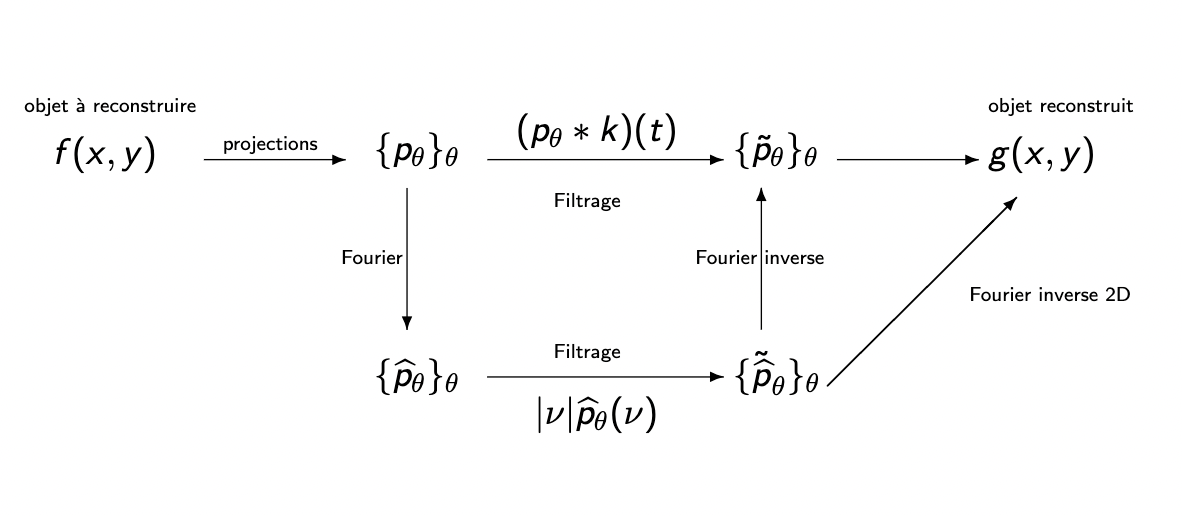
\includegraphics[scale = 0.6]{reconstrucfilterred.png}
    \caption{Rétroprojection filtrée}
\end{figure}
\newpage
\section{Discrétisation des méthodes analytiques}
En pratique il est impossible pour les machines de réaliser des projections $p_{\theta}$ pour tout $\theta \in [0,\pi]$.
De plus, pour un angle $\theta$ donné les projections $p_{\theta}$ sont connues que sur un ensemble discret de points.
On présente deux méthodes de discrétisation : 
\begin{enumerate}
    \item La première consiste à définir des opérateurs discrets analogues à ceux déjà étudiés (transformée de Radon, transformée de Fourier, rétroprojection...). Ensuite on appliquera les théorèmes démontrés 
    dans le cas continu aux outils discrets. 
    \item La deuxième méthode (souvent appelée transformée de Mojette) est une méthode algébrique. L'équation de projection est directement discrétisée et fournit ainsi un système d'équations linéaires. On est alors ramené 
    à un problème d'algèbre linéaire. 
\end{enumerate}
\subsection{Présentation de la première méthode}

Dans le but de donner l'équivalent discret du théorème de la coupe centrale \ref{coupe}, introduisons la transformée de Fourier discrète. 
\subsubsection{La transformée de Fourier discrète}

\begin{definition}[Transformée de Fourier discrète - 1D]
    Soit $f$ une fonction estimée aux points $(u_1, ... , u_N)$, on définit la transformée de Fourier discrète de $f$ par la suite $(F(u_1), ... , F(u_N))$
    où : $$\forall k \in \iintervalle{1}{N}, \; F(u_k) = \sum_{l = 1}^N f(u_l)\exp\left(\frac{-2i\pi k l}{N}\right)$$
\end{definition}
\begin{definition}[Transformée de Fourier discrète - 2D]
    Soit $f$ une fonction estimée aux points $(u_1, ... , u_N, v_1, ... , v_M)$ on définit la transformée de Fourier discrète 2D de $f$ par la suite double $(F(u_1, v_1), F(u_1, v_2), ... , F(u_N,v_M))$ où : 
    $$\forall k, l \in \iintervalle{1}{N} \times \iintervalle{1}{M}, F(u_k, u_l) = \sum_{n = 1}^N \sum_{m = 1}^M f(u_n,u_m) \mathrm{e}^{\frac{-2i \pi k n}{N}} \mathrm{e}^{\frac{-2i \pi l m}{M}} $$
\end{definition}
\noindent La transformée de Fourier discrète 1D peut aussi s'écrire matriciellement : 
    $$\begin{pmatrix}
        F(u_1) \\
        \vdots \\
        F(u_N)
    \end{pmatrix} =
        \Omega
        \begin{pmatrix}
            f(u_1) \\ \vdots \\ f(u_N)
        \end{pmatrix}\\
        \text{ avec } \Omega = (\omega^{kl})_{(k,l)} \text{ et } \omega = \mathrm{e}^{\frac{-2i\pi}{N}}$$
\begin{theorem}
    La matrice $\frac{\Omega}{\sqrt{N}}$ est unitaire.  
\end{theorem}
\begin{proof}
    $ \text{Soient } k,l \in \iintervalle{1}{N}$, 
    $$[\Omega^* \Omega]_{k,l} = \sum_{d = 1}^N [^t\overline{\Omega}]_{k,d} [\Omega]_{d,l} = \sum_{d = 1}^N \omega^{-kd} \omega^{dl} = \sum_{d= 1}^N \omega^{d(l-k)} = \delta_{k,l}N$$
    Donc : $$\left(\frac{\Omega}{\sqrt{N}}\right)^* \frac{\Omega}{\sqrt{N}} = I_N$$
\end{proof}
\noindent Conséquences : $\Omega$ est inversible et s'inverse facilement.
\begin{theorem}[Coupe centrale discret]
Soient $f$ la fonction caractéristique de notre objet, $\theta_k$ un angle échantillonné et $(u_l \cos(\theta_k), u_l \sin(\theta_k))$ un point d'une des droites d'échantillonage. On a : 
$$P_{\theta_k}(u_l) = F(u_l \cos \theta_k, u_l \sin \theta_k)$$
\end{theorem}

\subsection{Présentation de la deuxième méthode}
Nous définissons la matrice de projection : $P = (p_j)_j$ qui recense les valeurs des projections et la matrice de rétroprojection : $R = (R_{i,j})_{i,j}$ dont les valeurs sont expliquées sur le dessin. En notant $F$ le vecteur (colonne) des valeurs 
de $f$ sur les pixels, on a la relation matricielle : $P = RF$.\\
\begin{figure}[h]
    \centering
    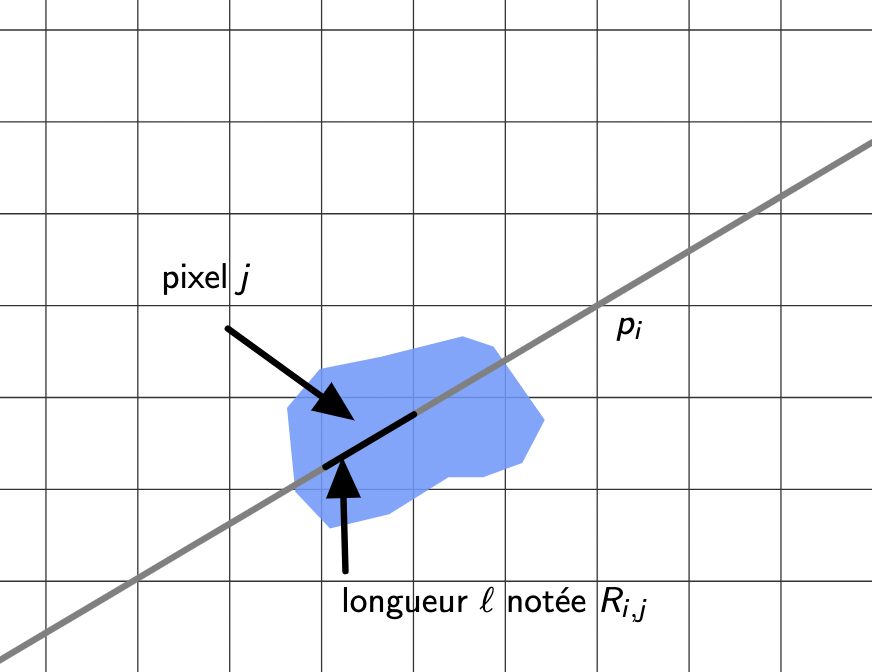
\includegraphics[scale = 0.5]{defObj.png}
\end{figure}

\subsubsection*{Reconstruction par la méthode ART}
En pratique nous avons donc accès aux matrices $P$ et $R$ et nous souhaitons accéder à la matrice $F$. La méthode employée est appelée : méthode ART ({\it Algebraic Reconstruction Technique }) ou méthode de Kaczmarz. 
Le principe de cette méthode est de partir d'un vecteur $F_0$ et de la modifier à chaque itération en le projettant sur un hyperplan affine. \\
\noindent On cherche à résoudre le système linéaire $P = RF$ d'inconnue $F$. Notons $L_1, ... , L_N$ les lignes de la matrice $R$, et pour $i \in \iintervalle{1}{N}, \; N_i = \;^t L_i$. La résolution du système est basé sur la résultat suivant :
\begin{theorem}
Soit $i \in \iintervalle{1}{N}$, on définit $\mathcal{H}_i$ l'hyperplan affine passant par $q_i = \frac{p_i}{\norme{N_i}^2}N_i$ et dirigé par $\{N_i\}^{\perp}$. $F$ est solution de $P = RF$ si et seulement si, $F \in \bigcap_{i = 1}^{N} \mathcal{H}_i$.
\end{theorem}

\noindent Alors, partant d'un vecteur $F_0$ quelconque, définissons par récurrence la suite $(F_k)_{k \in \N}$ qui aura pour but de converger vers la solution du système. 
\begin{itemize}
    \item on définit $F_1$ comme le projeté orthogonal de $F_0$ sur $\mathcal{H}_1$
    \item on définit $F_2$ comme le projeté orthogonal de $F_1$ sur $\mathcal{H}_2$
    \item ...
    \item on définit $F_N$ comme le projeté orthogonal de $F_{N-1}$ sur $\mathcal{H}_N$
    \item on recommence le processus à partir de $F_N$
\end{itemize}
On peut définir pour $i \in \iintervalle{1}{N}$ l'opérateur de projection orthogonale sur $\{N_i\}^{\perp}$ par $T_i = I_N - \frac{N_i}{\norme{N_i}^2}^t N_i$. \\
\noindent La suite $(F_k)_k$ est alors définie de la manière suivante : 
$$\left\{ 
    \begin{array}{ll}
        & F_0 \in M_{M,1}(\R)\\
        & \forall n \in \N^{*}, F_{n+1}= F_n - \frac{\scal{F_n - q_{r(n)+1}}{N_{r(n)+1}}}{\norme{N_{r(n)+1}}^2}N_{r(n)+1}  = T_{r(n)+1}(F_n) + q_{r(n)+1}
    \end{array}\right.$$
    où $r(n)$ est le reste de la division euclidienne de $n$ par $N$. 
\subsubsection*{Condition suffisante de convergence} 
Ensuite montrons qu'une condition suffisante de convergence est que la matrice $R$ est carrée inversible. Dans ce cas, l'intersection $\bigcap_{i = 1 }^N \mathcal{H}_i$ est composée d'un unique élément $\overline{F}$. Notons pour $n\in \N, \; \epsilon_n = F_n - \overline{F}$ l'erreur au rang $n$. Montrons que la suite $(\epsilon_n)_n$ converge vers $0$. 
\begin{proof}
    Soit $n\in \N$, $$\epsilon_{n+1} = F_{n+1} - \overline{F} = T_{r(n)+1}F_n - \overline{F} = T_{r(n)+1}(F_n - \overline{F}) = T_{r(n)+1}\epsilon_n$$
    car $\forall i \in \iintervalle{1}{N},\; \overline{F} \in \mathcal{H}_i$. 
    De plus, $T_{r(n) + 1}$ étant un opérateur de projection orthogonale on a d'après Pythagore $\forall x \in E, \norme{T_{r(n)+1}(x)} \leq \norme{x}$ on a alors : $\norme{\epsilon_{n+1}} \le \norme{\epsilon_n}$.\\
    Ainsi, la suite $(\norme{\epsilon_n})_n$ est décroissante et minorée. Elle converge donc et sa limite est la même que la suite extraite $(\norme{\epsilon_{nN+1}})_n$. Alors la suite $(\epsilon_n)_n$ est bornée et il existe une boule fermée $B$ qui contient cette suite. 
    Posons $T = T_N T_{N-1}\cdots T_1$. On a par récurrence immédiate : $\norme{\epsilon_{nN+1}} \le \normet{T}^n_B \norme{\epsilon_0}$.\\
    Montrons ensuite que $\normet{T}_B < 1$. \\
    Soit $x \in B$ : \\
    - S'il existe $i \in \iintervalle{0}{N-1}, T_i \cdots T_1 x \in \{N_{i+1}\}^{\perp}$ on a : 
    $$\norme{Tx} \le \normet{T_N} \cdots \normet{T_{i+2}}\norme{T_{i+1} \cdots T_1 x} \le \norme{T_{i+1} \cdots T_1 x} < \norme{T_{i} \cdots T_1 x} \le \norme{x} \text{ donc } \norme{Tx} < \norme{x}$$\\
    - Sinon $\forall i \in \iintervalle{0}{N-1}, T_i \cdots T_1 \in \{N_{i+1}\}^{\perp}$. Ainsi on a : $\forall i \in \iintervalle{0}{N-1}, T_i \cdots T_1 x = x$. \\
    Alors on a :
    $\forall i \in \iintervalle{1}{N}, \scal{N_i}{x} = 0$ et $(N_1, ... , N_N)$ est une base de $E$ car $R$ est inversible.\\ Donc $x = 0$
    si bien que $\forall x \in B - \{0\}, \norme{Tx} < \norme{x}$ et puisque $B$ est compacte (dimension finie) on a en passant au sup $\normet{T}_B < 1$. On peut alors conclure que $\epsilon_{nN+1} \underset{n_{\infty}}{\longrightarrow} 0$ donc $\epsilon_n \underset{n_{\infty}}{\longrightarrow} 0$ si bien que $(F_n)_n$ converge. 
\end{proof}
\definecolor{uuuuuu}{rgb}{0.26666666666666666,0.26666666666666666,0.26666666666666666}
\definecolor{ududff}{rgb}{0.30196078431372547,0.30196078431372547,1}
\definecolor{cqcqcq}{rgb}{0.7529411764705882,0.7529411764705882,0.7529411764705882}
\begin{center}
\begin{tikzpicture}[line cap=round,line join=round,>=triangle 45,x=1cm,y=1cm]
\draw [color=cqcqcq,, xstep=0.5cm,ystep=0.5cm] (-6.825738728170894,-3.323643197569457) grid (7.179318629864831,5.802748875211437);
\clip(-6.825738728170894,-3.323643197569457) rectangle (7.179318629864831,5.802748875211437);
\draw [line width=1pt,domain=-6.825738728170894:7.179318629864831] plot(\x,{(--16.872505481862348--3.2990555973059905*\x)/8.379958609883893});
\draw [line width=1pt,domain=-6.825738728170894:7.179318629864831] plot(\x,{(--13.86462588822425-7.815411248291108*\x)/-5.733656470634804});
\draw [line width=1pt,domain=-6.825738728170894:7.179318629864831] plot(\x,{(-16.872505481862348-3.2990555973059905*\x)/-8.379958609883893});
\draw (-6,0.5) node[anchor=north west] {$\mathcal{H}_1$};
\draw (0.9,-1) node[anchor=north west] {$\mathcal{H}_2$};
\draw[color=ududff] (-4.48860034926011,2.919093346859538) node {$F_{0}$};
\draw [fill=ududff] (-4.58474,2.7017) circle (2.5pt);
\draw [line width=1pt] (-4.58474,2.7017)-- (-3.7349172900658614,0.5430582539188338);
\draw [fill=ududff] (-3.7349172900658614,0.5430582539188338) circle (2pt);
\draw[color=ududff] (-3.67104623952706,0.8130028685254858) node {$F_{1}$};
\draw [line width=1pt] (-3.7349172900658614,0.5430582539188338)-- (0.10545370652402351,-2.2743709656952342);
\draw [fill=ududff] (0.10545370652402351,-2.2743709656952342) circle (2pt);
\draw[color=ududff] (0.13,-1.9) node {$F_{2}$};   
\draw [line width=1pt] (-1.3702205530839788,1.474001516200577)-- (0.10545370652402351,-2.2743709656952342);
\draw [fill=ududff] (-1.3702205530839788,1.474001516200577) circle (2pt);
\draw[color=ududff] (-1.4316588954756626,1.7638538439758806) node {$F_{3}$};
\draw [line width=1pt] (-1.3702205530839788,1.474001516200577)-- (1.3768577222169673,-0.541350283995937);
\draw [line width=1pt] (0.3212845227553587,2.1399199948118426)-- (1.3768577222169673,-0.541350283995937);
\draw [line width=1pt] (0.3212845227553587,2.1399199948118426)-- (2.2863131768440894,0.6983068922432208);
\draw [line width=1pt] (1.5312449277593612,2.6162620428428394)-- (2.2863131768440894,0.6983068922432208);
\draw [line width=1pt] (1.5312449277593612,2.6162620428428394)-- (2.936861085881669,1.585053329160751);
\draw [line width=1pt] (2.936861085881669,1.585053329160751)-- (2.3967487932745164,2.9569970637354195);
\draw [line width=1pt] (2.3967487932745164,2.9569970637354195)-- (3.4022083217467656,2.2193571177061076);
\draw [line width=1pt] (3.4022083217467656,2.2193571177061076)-- (3.015857433626426,3.2007302276301);
\draw [line width=1pt] (3.015857433626426,3.2007302276301)-- (3.7350785791389494,2.6730846765803147);
\draw [line width=1pt] (3.7350785791389494,2.6730846765803147)-- (3.458715662029889,3.3750764249375953);
\draw [line width=1pt] (3.458715662029889,3.3750764249375953)-- (3.9731859529806637,2.9976431947535453);
\draw [line width=1pt] (3.9731859529806637,2.9976431947535453)-- (3.775499175749186,3.499789024691639);
\draw [line width=1pt] (3.775499175749186,3.499789024691639)-- (4.143507933448267,3.22980504972257);
\draw [fill=ududff] (1.3768577222169673,-0.541350283995937) circle (2pt);
\draw[color=ududff] (1.7,-0.4844199577900065) node {$F_{4}$};
\draw [fill=ududff] (0.3212845227553587,2.1399199948118426) circle (2pt);
\draw[color=ududff] (0.29231390113533406,2.394792341704647) node {$F_{5}$};
\draw [fill=ududff] (2.2863131768440894,0.6983068922432208) circle (2pt);
\draw[color=ududff] (2.55,0.7152518336660993) node {$F_{6}$};
\draw [fill=ududff] (4.57147,3.81315) circle (2pt);
\draw[color=ududff] (4.557813604090376,4.012127645741768) node {$\overline{F}$};
\draw [fill=ududff] (1.5312449277593612,2.6162620428428394) circle (2pt);
\draw[color=ududff] (1.509758608020419,2.892433973716069) node {$F_{7}$};
\draw [fill=ududff] (2.936861085881669,1.585053329160751) circle (2pt);
\draw[color=ududff] (3.3,1.5772382319715976) node {$F_{8}$};
\draw [fill=ududff] (2.3967487932745164,2.9569970637354195) circle (2pt);
\draw[color=ududff] (2.327312717753469,3.247892282295656) node {$F_{9}$};
\draw [fill=ududff] (3.4022083217467656,2.2193571177061076) circle (2pt);
\draw[color=ududff] (3.8,2.1992902719858747) node {$F_{10}$};
\draw [fill=ududff] (3.015857433626426,3.2007302276301) circle (2pt);
\draw[color=ududff] (2.9404783000532566,3.478940182872387) node {$F_{11}$};
\draw [fill=ududff] (3.7350785791389494,2.6730846765803147) circle (2pt);
\draw[color=ududff] (4.4,3) node {$F_{14}$};
\draw [fill=ududff] (3.458715662029889,3.3750764249375953) circle (2pt);
\draw [fill=ududff] (3.9731859529806637,2.9976431947535453) circle (2pt);
\draw[color=ududff] (4.6,3.3) node {$F_{16}$};
\draw [fill=ududff] (3.775499175749186,3.499789024691639) circle (2pt);
\draw [fill=ududff] (4.143507933448267,3.22980504972257) circle (2pt);
\draw [fill=ududff] (3.7754991757491845,3.4997890246916397) circle (2pt);
\draw[color=ududff] (3.820237613787734,3.827760998878098) node {$F_{15}$};
\draw [fill=ududff] (3.458715662029889,3.3750764249375953) circle (2pt);
\draw[color=ududff] (3.420347016635699,3.647782879447691) node {$F_{13}$};
\draw [fill=ududff] (3.73507857913895,2.6730846765803142) circle (2pt);
\draw[color=ududff] (4.2,2.6969319039972963) node {$F_{12}$};
\end{tikzpicture}
Illustration de la méhode en dimension 2 
\end{center}

\end{document}
